\documentclass[tikz,border=6pt]{standalone}
\usepackage{tikz}
\usetikzlibrary{arrows.meta,patterns}
\definecolor{nebula}{HTML}{6366F1}
\definecolor{spark}{HTML}{14B8A6}
\definecolor{ink}{HTML}{334155}
\begin{document}
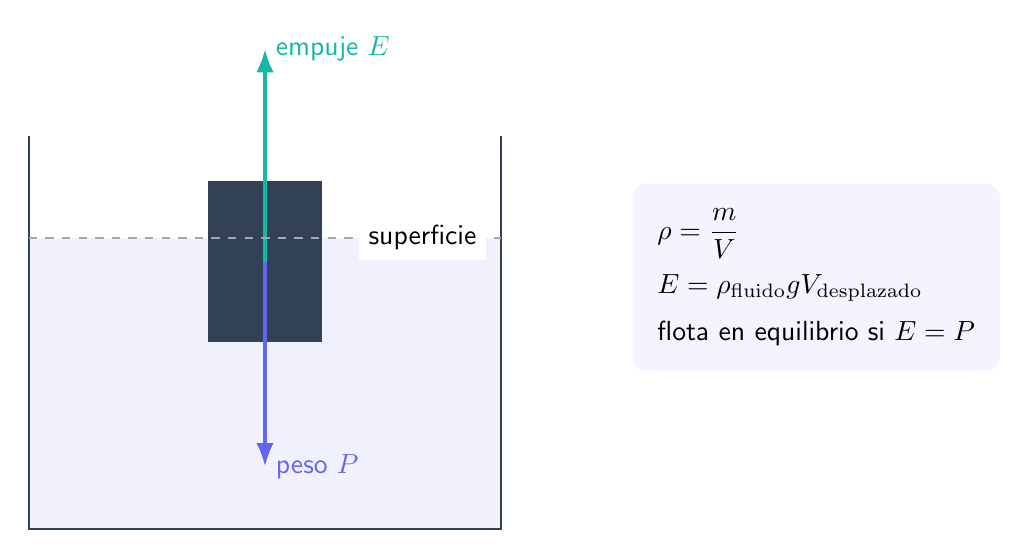
\begin{tikzpicture}[font=\sffamily,>=Latex]
  \fill[nebula!9] (0,0) rectangle (6,3.7);
  \draw[thick,ink] (0,5)--(0,0)--(6,0)--(6,5);
  \draw[fill=white,very thick,ink] (2.3,2.4) rectangle (3.7,4.4);
  \draw[->,very thick,spark] (3,3.4)--(3,6.1) node[right] {empuje $E$};
  \draw[->,very thick,nebula] (3,3.4)--(3,0.8) node[right] {peso $P$};
  \draw[dashed,ink!45] (0,3.7)--(6,3.7);
  \node[fill=white] at (5,3.7) {superficie};
  \node[align=left,fill=nebula!7,rounded corners=5pt,inner sep=9pt] at (10,3.2) {$\displaystyle \rho=\frac{m}{V}$\\[5pt]$\displaystyle E=\rho_{\rm fluido}gV_{\rm desplazado}$\\[5pt]flota en equilibrio si $E=P$};
\end{tikzpicture}
\end{document}
